\documentclass[a4paper,12pt,fleqn]{article}
\usepackage[T1]{fontenc}
\usepackage{ucs}
\usepackage[utf8x]{inputenc}
\usepackage{ngerman}
\usepackage[ngerman]{babel}
\usepackage{lastpage}
\usepackage[pdftex]{color,graphicx}
\usepackage{listings}
\usepackage{pdflscape}
\usepackage{longtable}
\usepackage[inner=2cm,outer=2cm,top=1cm,bottom=1.5cm,includeheadfoot]{geometry}
\usepackage{fancyhdr}
\usepackage{url}
\usepackage{draftwatermark}
\usepackage{booktabs}
\usepackage{blindtext} 
\usepackage{framed} 
\usepackage{xcolor} 
\colorlet{shadecolor}{black} 
\usepackage{latexsym}

\usepackage{bbm}
\usepackage{enumitem}

\SetWatermarkText{Vertraulich}
\SetWatermarkScale{4}
\SetWatermarkLightness{0.9}

\usepackage{pgfgantt}
\usepackage{amsmath,amssymb,amsfonts,amstext}
\usepackage{floatflt}
\usepackage{tikz}
\usetikzlibrary[arrows,snakes,backgrounds,shapes]
\usetikzlibrary{through}
\usetikzlibrary{calc}
\usepackage{caption}
\usepackage{subcaption}

% highlighting
\usepackage{xcolor,soul}

%---- PageLayout
\pagestyle{fancy}

\setlength{\headsep}{10mm}

\usepackage{eso-pic}

%----------------------------------------------------------------------------
% HEADER --------------------------------------------------------------------
%----------------------------------------------------------------------------
\fancyhead[R]{
  
\includegraphics[width=100pt,keepaspectratio]{img/amedo2012.png}
}

\fancyhead[C]{ Wochenbericht KW 30 }

\fancyhead[L]{
  \begin{tabular}[b]{l}
  Christoph Gnip\\
  Projekt: PRPS-Evolution
  \end{tabular}
}

%Linie oben
\renewcommand{\headrulewidth}{0.5pt}
%----------------------------------------------------------------------------

%----------------------------------------------------------------------------
%----------------------------------------------------------------------------
%----------------------------------------------------------------------------
\fancyfoot[L]{Stand: \today}
\fancyfoot[C]{ EXTERN }
\fancyfoot[R]{\thepage{} von \pageref{LastPage}}

% Linie unten
\renewcommand{\footrulewidth}{0.5pt}
%----------------------------------------------------------------------------

% Import Macros  ------------------------------------------------------------
\newcommand\nn{\newline\newline}

%----------------------------------------------------------------------------
% Start the Document --------------------------------------------------------
%----------------------------------------------------------------------------
\begin{document}

\setlength{\headheight}{36pt}

\begin{titlepage}


%- the Title page --------------------------------------------------------
\begin{center}
%\vspace*{2.5cm}
{\Huge \textbf{Wochenbericht KW 30}\par}
\vspace{1cm}
{\Huge 22.7. - 28.7.2013\par}
\vspace{1cm}
{\Huge Projektwoche: 14\par}

\vspace{2cm}

\large{Erstellt durch}\\
\Large{\textbf{Christoph Gnip}}

\vspace{4cm}

\Large{\textbf{Extern}}

\vfill

{\normalsize Fachbereich Elektrotechnik und angewandte Naturwissenschaften\\
Westfälische Hochschule\\[2ex]Juni 2013}

\end{center}
\newpage

\end{titlepage}

%- Section 1 ----------------------------------------------------------------
\section[Allgemeines]{Allgemeines}
%
%- Section 2 ----------------------------------------------------------------
\section[Fortschritt]{Projektfortschritt}
%
In dieser Woche wurden die Arbeiten an der Visualisierung und intensiviert. Es gelang eine gut Darstellungsmethode für die Ergebnisse des Optimierung zu erarbeiten. Die Darstellung ist von den vorgeschlagenen in \cite{Hansen:2,Hansen:3} inspiriert und ermöglicht eine Vergleichbarkeit verschiedener Algorithmen, Parameter und Ergebnisse.
%
%- Section 2.1 --------------------------------------------------------------
\subsection{Programmierung}
%
Das Programm wurde um weitere Optionen und Übergabeparameter erweitert. Es ermöglicht eine automatische Generierung der Ausgabedateien mehrere Lösungen, die bereits für eine Weiterverarbeitung und Darstellung Konfektioniert sind. Im Weiteren kann nun dynamisch Einfluss auf die CMA-ES-Parameter $\mu$ und $\lambda$ genommen werden. Diese sind als Übergabeparameter realisiert und werden an die entsprechen Funktionen weitergegeben. 
%
%- Section 2.2 --------------------------------------------------------------
\subsection{Visualisierung}
%
Für die Visualisierung der Daten wurden die in Anhang~\ref{lst:gnuplot_script} und Anhang~\ref{lst:cp_script} gezeigten Skripte erstellt. Das Skript aus Anhang~\ref{lst:cp_script} dient der einfachen Kopierung der Daten. Zusätzlich wird via \textit{sed} die erste Zeile entfernt. In dieser Zeile steht die verwendete Antennenkonfiguration, diese kann verworfen werden. Das Gnuplot-Skript in Anhang~\ref{lst:gnuplot_script} erstellt aus den Eingabedaten im Anschluss die entsprechenden Plots. Die Plots sind in Anhang~\ref{lst:plots} gezeigt.
%- Section 2.3 --------------------------------------------------------------
\subsection{Shark 3.0b}
%
Es wird im Zusammenhang mit der Optimierung ein Fehlverhalten beobachtet, es konnte zum jetzigen Zeitpunkt noch nicht eindeutig lokalisiert werden. Es zeigt sich, dass einige Funktionen in der Library nicht den erwarteten Rückgabewert liefern. Voraussichtlich in der nächsten Woche können diese Fehler behoben werden. Dort wird Zeit zur Verfügung stehen um die Funktionen der Library genauer zu untersuchen.
%
%- Section 3 -----------------------------------------------------------------
\section{Probleme}
\label{Problems}
%
Die Erstellung des gnuplot Skriptes hat längere Zeit in Anspruch genommen als erwartet. Aufgrund dieser Tatsache konnten die geplanten Experimente mit den Algorithmus und den Auswirkungen verschiedener Parameter nicht mehr durchgeführt werden und werden auf nächste Woche verschoben. Es ist immer noch nicht gelungen eine gute Beschriftung für den Plot der freien Parameter (Abbildung~\ref{fig:ResA20}) einzuführen.
%
%- Appendix ------------------------------------------------------------------
%
%
%
\begin{appendix}

%----------------------------------------------------------------------------
%----------------------------------------------------------------------------
%----------------------------------------------------------------------------
\newpage

\begin{center}
	\huge{Anhänge}
\end{center}

\normalsize

%----------------------------------------------------------------------------
%----------------------------------------------------------------------------
%----------------------------------------------------------------------------
\begin{landscape}
\section{Beispiel Plots}
\label{lst:plots}
\begin{figure} [h]
         \centering
         \caption{ Darstellung der von Gnuplot erzeugten Plots. Ausgewählt wurden zufällig 2 aus 50 durchgeführten Lösungen. Pro Reihe ist jeweils das Ergebnis einer Lösung dargestellt. Auf Basis dieser Plots kann eine Beurteilung der Modellgüte und eine Untersuchung der Einflüsse durch Optimierungsparameter durchgeführt werden. Diese werden in der kommenden Woche durchgeführt. }
%         \label{fig:3}
%         
         \begin{subfigure}[t]{0.34\textwidth}
                 \centering
                 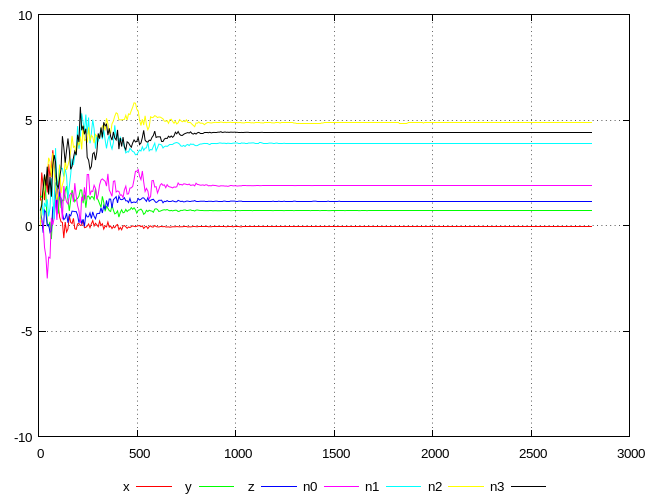
\includegraphics[width=\textwidth]{common/img/objectVar0.png}
                 \label{fig:ResA0}\textit{}
         \end{subfigure}
%         
\qquad
         \begin{subfigure}[t]{0.34\textwidth}
                 \centering
                 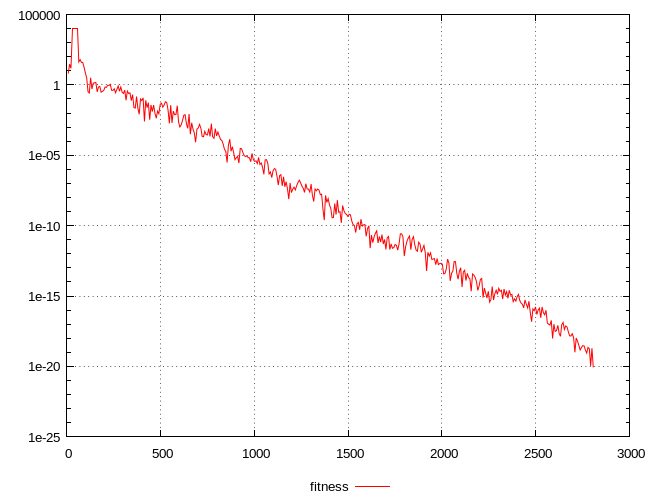
\includegraphics[width=\textwidth]{common/img/fitness0.png}
                 \label{fig:ResB0}
         \end{subfigure}
%
\qquad
         \begin{subfigure}[t]{0.34\textwidth}
                 \centering
                 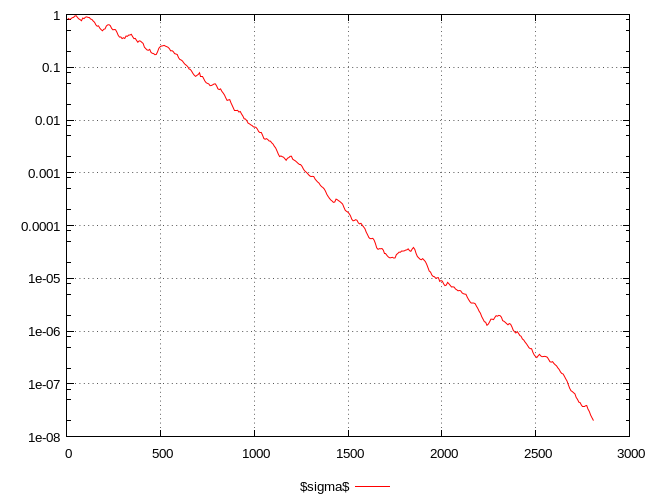
\includegraphics[width=\textwidth]{common/img/sigma0.png}
                 \label{fig:ResC0}
         \end{subfigure}
\\
         \begin{subfigure}[t]{0.34\textwidth}
                 \centering
                 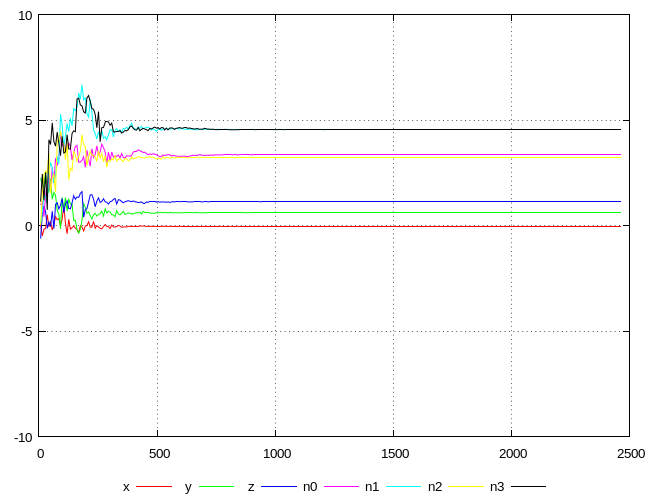
\includegraphics[width=\textwidth]{common/img/objectVar20.png}
%                 \vspace{.1cm}
                 \caption{ Verlauf der optimierten Parameter; Bei diesem Modell wurden 7 freie Parameter optimiert. }
                 \label{fig:ResA20}\textit{}
         \end{subfigure}
%         
\qquad
         \begin{subfigure}[t]{0.34\textwidth}
                 \centering
                 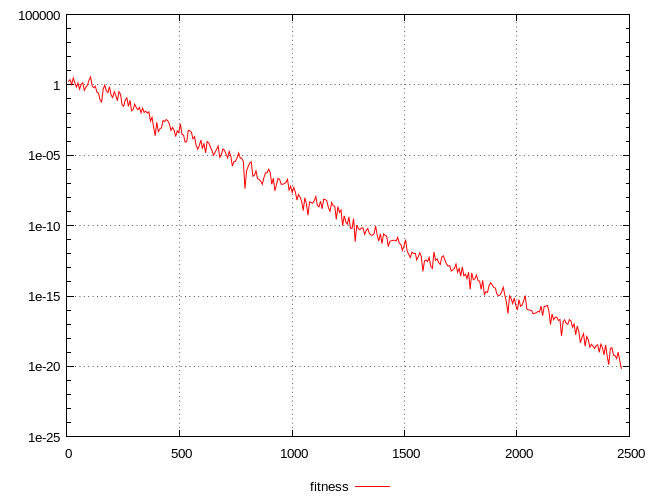
\includegraphics[width=\textwidth]{common/img/fitness20.png}
%                 \vspace{.1cm}
                 \caption{ Verlauf der Fitness der Lösung; Das Abruchkriterium wurde auf $\epsilon<10^-21$ eingestellt }
                 \label{fig:ResB20}
         \end{subfigure}
%
\qquad
         \begin{subfigure}[t]{0.34\textwidth}
                 \centering
                 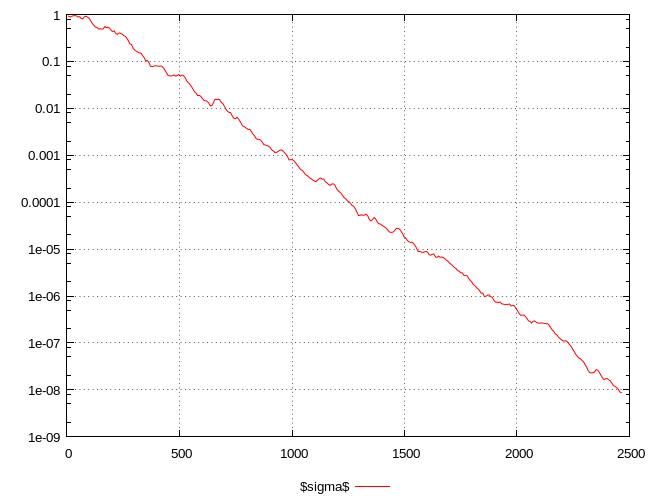
\includegraphics[width=\textwidth]{common/img/sigma20.png}
%                 \vspace{.1cm}
                 \caption{ Verlauf von $\sigma$ während der Lösung; Sigma steuert unmittelbar die Schrittweite des Algorithmus }
                 \label{fig:ResC20}
         \end{subfigure}
\end{figure}
\end{landscape}

%----------------------------------------------------------------------------
%----------------------------------------------------------------------------
%----------------------------------------------------------------------------
\begin{landscape}
\section{Gnuplot Skript}
\label{lst:gnuplot_script}

% listings print source code

% define colors for source code list
\definecolor{colKeys}{rgb}{0,0,1}
\definecolor{colIdentifier}{rgb}{0,0,0}
\definecolor{colComments}{rgb}{0,1,0.3}
\definecolor{colString}{rgb}{0,0.5,0}

\definecolor{dkgreen}{rgb}{0,0.6,0}
\definecolor{gray}{rgb}{0.5,0.5,0.5}

\lstset{language=Matlab,
   keywords={break,case,catch,continue,else,elseif,end,for,function,
   global,if,otherwise,persistent,return,switch,try,while,ones,zeros},
   float=hbp,
   basicstyle=\ttfamily\small,
   identifierstyle=\color{colIdentifier},
   keywordstyle=\color{blue},
   commentstyle=\color{dkgreen},
   stringstyle=\color{red},
   columns=flexible,
   tabsize=2,
   frame=single,
   numbers=left,
   extendedchars=true,
   showspaces=false,
   numberstyle=\tiny\color{gray},
   stepnumber=1,
   numbersep=10pt,
   showspaces=false,
   showstringspaces=false,
   breakautoindent=true}

\lstinputlisting[language=Gnuplot,
		numbers=left,
		frameround=fttt,
		frame=trbl,
		xleftmargin=1cm]{common/src/generate_cma_plot.gp}

\end{landscape}

%----------------------------------------------------------------------------
%----------------------------------------------------------------------------
%----------------------------------------------------------------------------
\begin{landscape}
\section{Bash Kopier-Skript}
\label{lst:cp_script}

% listings print source code

% define colors for source code list
\definecolor{colKeys}{rgb}{0,0,1}
\definecolor{colIdentifier}{rgb}{0,0,0}
\definecolor{colComments}{rgb}{0,1,0.3}
\definecolor{colString}{rgb}{0,0.5,0}

\definecolor{dkgreen}{rgb}{0,0.6,0}
\definecolor{gray}{rgb}{0.5,0.5,0.5}

\lstset{language=Matlab,
   keywords={break,case,catch,continue,else,elseif,end,for,function,
   global,if,otherwise,persistent,return,switch,try,while,ones,zeros},
   float=hbp,
   basicstyle=\ttfamily\small,
   identifierstyle=\color{colIdentifier},
   keywordstyle=\color{blue},
   commentstyle=\color{dkgreen},
   stringstyle=\color{red},
   columns=flexible,
   tabsize=2,
   frame=single,
   numbers=left,
   extendedchars=true,
   showspaces=false,
   numberstyle=\tiny\color{gray},
   stepnumber=1,
   numbersep=10pt,
   showspaces=false,
   showstringspaces=false,
   breakautoindent=true}

\lstinputlisting[language=bash,
		numbers=left,
		frame=trbl,
		xleftmargin=1cm]{common/src/copy_data_to_printable.sh}

\end{landscape}

%----------------------------------------------------------------------------
%----------------------------------------------------------------------------
%----------------------------------------------------------------------------
\newpage
\begin{landscape}
	\section{Projektlaufplan KW 30}
	\label{sec:projectplan}
	\scalebox{.75}{
		\begin{ganttchart}[vgrid={draw=none,*1{gray, dashed}},
				hgrid=true,
				today=30,
				title height=1,
				y unit title=0.6cm,
				y unit chart=0.8cm,
				group right shift=0,
				group top shift=.3,
				group height=.3,
				milestone width=.8,
				group peaks={}{}{.2},
				incomplete/.style={fill=black!15}, %
				bar/.style={fill=white}, %
				today label={Heute},
				today rule/.style={dashed, thick}]{44}


\gantttitle{\textbf{2013}}{44} \\
\gantttitlelist{16,...,37}{2} \\
%-------------------------------------------------------------
\ganttgroup{Projekt Evaluation}{3}{14} \\
\ganttbar[progress=100, progress label font=\small\color{black!75},
	progress label anchor/.style={right=4pt}]{Installation der Umgebungen}{3}{6} \\
	
\ganttbar[progress=100, progress label font=\small\color{black!75},
	progress label anchor/.style={right=4pt},
	bar label font=\normalsize\color{black},
	name=rech]{Recherche}{3}{7} \\
	
\ganttmilestone[name=ms1]{Vorstellung der Ergebnisse}{7} \\
	
\ganttbar[progress=99, progress label font=\small\color{black!75},
	progress label anchor/.style={right=4pt},
	bar label font=\normalsize\color{black},
	name=pflichten]
	{Pflichtenheft}{5}{8} \\
	
\ganttmilestone[name=ms2]{Pflichtenheft fertig}{8} \\

\ganttbar[progress=100, progress label font=\small\color{black!75},
	progress label anchor/.style={right=4pt},
	bar label font=\normalsize\color{black},
	name=bNumVerf]
	{Einarbeitung num. Verfahren}{5}{16} \\

\ganttbar[progress=95, progress label font=\small\color{black!75},
	progress label anchor/.style={right=34pt},
	bar label font=\normalsize\color{black},
	name=bCMAES]
	{speziell CMA-ES}{7}{10} \\

\ganttmilestone[name=ms3]{Beurteilung num. Verfahren}{16} \\

\ganttlinkedbar[progress=100, progress label font=\small\color{black!75},
	progress label anchor/.style={right=34pt},
	bar label font=\normalsize\color{black}]
	{Shark Einarbeitung}{17}{18} \\

\ganttlinkedmilestone[name=ms7]{Abschluss Evaluation}{18} \\
	
%-------------------------------------------------------------
\ganttgroup{Erstellung Prototyp}{15}{26} \\
\ganttgroup{(optional)}{15}{18} \\
\ganttbar[progress=100, progress label font=\small\color{black!75},
	progress label anchor/.style={right=4pt},
	bar label font=\normalsize\color{black}]
	{(Entwurf digi. Filter)}{15}{15} \\

\ganttlinkedbar[progress=90, progress label font=\small\color{black!75},
	progress label anchor/.style={right=4pt},
	bar label font=\normalsize\color{black},
	name=bImpFPGA]
	{(Implementation FPGA)}{16}{18} \\

\ganttmilestone[name=ms4]{(Verifikation dig. Filter)}{18} \\
	
\ganttbar[progress=99, progress label font=\small\color{black!75},
	progress label anchor/.style={right=4pt},
	bar label font=\normalsize\color{black},
	name=bImplAlgo]
	{Implementation Algorithmus}{15}{26} \\

\ganttlinkedmilestone[name=ms5]{Implementation Done}{26} \\

%-------------------------------------------------------------
\ganttgroup{Verifikation}{27}{34} \\
\ganttbar[progress=50, progress label font=\small\color{black!75},
	progress label anchor/.style={right=4pt},
	bar label font=\normalsize\color{black},
	name=bVerf]
	{Durchf\"uhrung Verifikation}{27}{34} \\

\ganttlinkedmilestone[name=ms6]{Verifikation Done}{34} \\

%-------------------------------------------------------------
\ganttgroup{Projektdokumentation}{35}{42} \\

\ganttbar[progress=0, progress label font=\small\color{black!75},
	progress label anchor/.style={right=4pt},
	bar label font=\normalsize\color{black},
	name=thesis]
	{Thesis schreiben}{35}{42} \\
	
\ganttmilestone[name=msthesis,milestone label font=\color{red}, 
	milestone/.style={fill=red}]{Abgabe}{42}

%\ganttlink{ms7}{bImplAlgo}
\ganttlink{bImpFPGA}{ms4}
\ganttlink{bNumVerf}{ms3}
\ganttlink{bCMAES}{ms3}
\ganttlink{rech}{ms1}
\ganttlink{pflichten}{ms2}
\ganttlink{thesis}{msthesis}

	\end{ganttchart}
		}
\end{landscape}

%----------------------------------------------------------------------------

\end{appendix}


\newpage
%- Bibliography --------------------------------------------------------------
\bibliographystyle{ieeetr}
\bibliography{../bib/mathesis_collection1}

\end{document}